\documentclass[aspectratio=169, hyperref={colorlinks, linkcolor=beamer@centricgreen}, urlcolor=links]{beamer}

% Must be loaded first
\usepackage{tikz}
\usetikzlibrary{shapes,arrows,positioning,fit,calc}

\usepackage[utf8]{inputenc}
\usepackage{textpos}

% Font configuration
\usepackage{fontspec}

\usepackage[listings, minted]{tcolorbox}
\usepackage{smartdiagram}
\usepackage[export]{adjustbox}

\input{font.tex}

% Tikz for beautiful drawings
\usetikzlibrary{mindmap,backgrounds}
\usetikzlibrary{arrows.meta,arrows}
\usetikzlibrary{shapes.geometric}

% Minted configuration for source code highlighting
\usepackage{minted}
\setminted{highlightcolor=orange!30, linenos}
\setminted{style=lovelace}

\usepackage[listings, minted]{tcolorbox}
\tcbset{left=6mm}

% Use the include theme
\usetheme{codecentric}

% Metadata
\title{Free vs Final Tagless}
\author{Markus Hauck (@markus1189)}

% The presentation content
\begin{document}

\begin{frame}[noframenumbering,plain]
  \titlepage{}
\end{frame}

\section{Introduction}\label{sec:introduction}

\begin{frame}
  \begin{center}
    {\Huge Free vs Tagless}
  \end{center}
\end{frame}

\begin{frame}[fragile]
  \frametitle{Content}
  \begin{itemize}
  \item start with the basics from Oleg's excellent paper
  \item \href{http://okmij.org/ftp/tagless-final/course/index.html}{Typed tagless-final interpretations: Lecture notes}
  \item clarify tagged, tagless, initial and final
  \item extensibility
  \item inspection and transformation of programs
  \item Free-X and MTL vs initial and final
  \item comparison of both approaches
  \end{itemize}
\end{frame}

\begin{frame}
  \begin{center}
    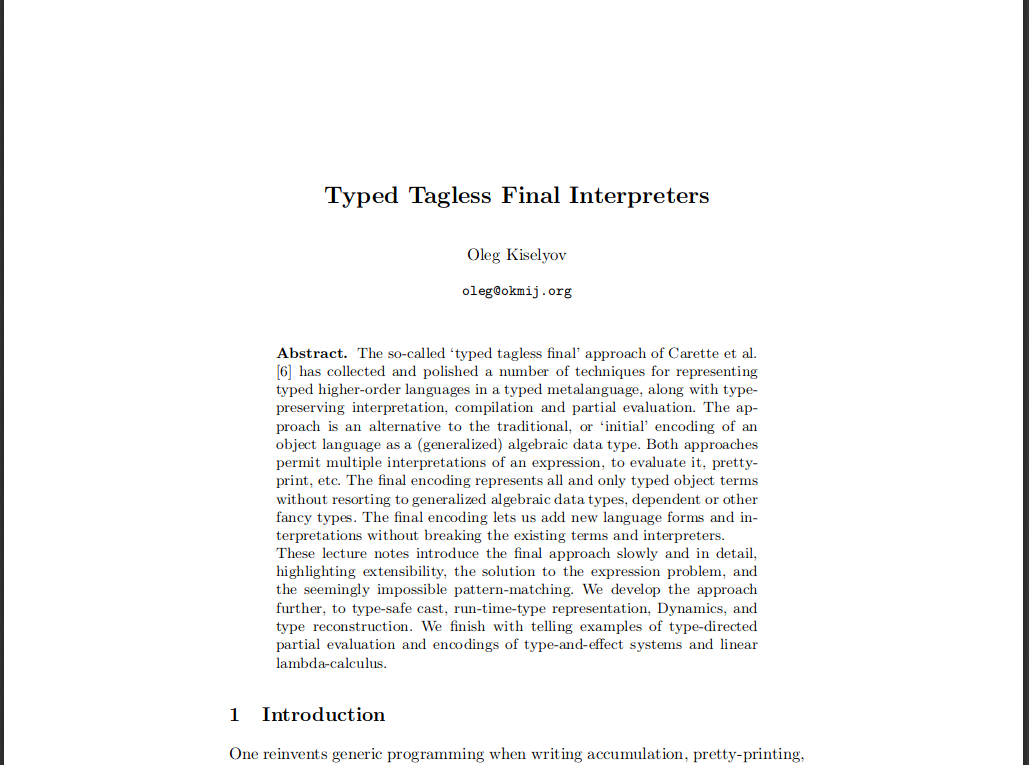
\includegraphics[width=0.5\textwidth]{static-images/final-tagless.png}
    \vfill
    \href{http://okmij.org/ftp/tagless-final/course/index.html}{http://okmij.org/ftp/tagless-final/course/index.html}
  \end{center}
\end{frame}

\begin{frame}
  \frametitle{The Toy Language}
  \begin{itemize}
  \item toy language with operations:
  \item integer constants: \texttt{Int(42)}
  \item integer addition: \texttt{Int(21) + Int(21)}
  \item string constants: \texttt{Str("4")}
  \item string concatenation: \texttt{Str("4") + Str("2")}
  \item conversion from string to integer: \texttt{StrToInt("42")}
  \end{itemize}
\end{frame}

\section{Initial vs Final vs Tagged}\label{sec:initial-final-tagged}

\begin{frame}
  \begin{center}
    \Huge
    Initial vs Final vs Tagged
  \end{center}
\end{frame}

\begin{frame}
  \frametitle{Terminology}

  directly from the \href{http://okmij.org/ftp/tagless-final/course/lecture.pdf}{paper} by Oleg Kiselyov:
  \vfill
  \begin{quote}
    There are \textbf{two basic approaches} to embedding languages and
    writing their interpreters, which we shall call, somewhat
    informally, \textbf{initial} and \textbf{final}.
  \end{quote}
  \vfill
  \begin{quote}
    The \textbf{initial} approach represents a term of an object
    language \textbf{as a value} of an algebraic data type in the
    metalanguage; interpreters recursively traverse the values
    de-constructing them by \textbf{pattern-matching}.
  \end{quote}
  \vfill
  \begin{quote}
    In the \textbf{final} approach, object language terms are
    represented as expressions built from a small set of
    \textbf{combinators}, which are \textbf{ordinary functions} rather
    than data constructors.
  \end{quote}
\end{frame}

\begin{frame}[fragile]
  \frametitle{Interpreter: Initial Tagged}
  \begin{itemize}
  \item small language: addition, concatenation, literals and conversion from string to int
  \end{itemize}
  \begin{minted}{scala}
    1 + 1
    "hello," + " world"
    "42".toInt
  \end{minted}
\end{frame}

\begin{frame}[fragile]
  \frametitle{Interpreter: Initial Tagged}
  \inputminted[fontsize=\footnotesize]{scala}{snippets/initial-tagged-expr.scala}
\end{frame}

\begin{frame}[fragile]
  \frametitle{Interpreter: Initial Tagged}
  \inputminted[fontsize=\footnotesize]{scala}{snippets/initial-tagged-sample.scala}
\end{frame}

\begin{frame}[fragile]
  \frametitle{Interpreter: Initial Tagged}
  \inputminted[fontsize=\footnotesize]{scala}{snippets/initial-tagged-interp-wrong.scala}
\end{frame}

\begin{frame}[fragile]
  \frametitle{Interpreter: Initial Tagged}
  \inputminted[fontsize=\footnotesize]{scala}{snippets/initial-tagged-result.scala}
  \vspace{5mm}
  \inputminted[fontsize=\footnotesize]{scala}{snippets/initial-tagged-interp.scala}
\end{frame}

\begin{frame}[fragile]
  \frametitle{Interpreter: Initial Tagged}
  \inputminted[fontsize=\footnotesize]{scala}{snippets/initial-tagged-add.scala}
\end{frame}

\begin{frame}[fragile]
  \frametitle{Interpreter: Initial Tagged}
  \begin{itemize}
  \item problems: have to handle errors in interpreter
  \item should: don't allow invalid programs at all
  \item btw: this is a very nice criteria for \texttt{any} DSL
  \end{itemize}
\end{frame}

\begin{frame}
  \frametitle{Tagged Initial Encoding}
  \begin{itemize}
  \item initial encoding = data structure + \texttt{Result} union + error handling
  \item ``tagged union'' a.k.a.\ sum types in type theory
  \item this ``tag'' is used for pattern matching
  \item programs are first class, store as data etc
  \end{itemize}
\end{frame}

\begin{frame}
  \frametitle{Tagless Initial Encoding}
  \begin{itemize}
  \item we saw the problem of invalid programs
  \item next step: make invalid programs impossible
  \item Use GADTs: ADTs that refine the type parameter
  \end{itemize}
\end{frame}

\begin{frame}[fragile]
  \frametitle{Interpreter: Initial Tagless}
  \inputminted[highlightlines={1}, fontsize=\footnotesize]{scala}{snippets/initial-tagless-expr.scala}
  \begin{itemize}
  \item \texttt{Expr} has a type parameter that is refined in subclasses
  \item when pattern matching, we can recover this refinement
  \end{itemize}
\end{frame}

\begin{frame}[fragile]
  \frametitle{Interpreter: Initial Tagless}
  \inputminted[fontsize=\footnotesize]{scala}{snippets/initial-tagless-sample.scala}
\end{frame}

\begin{frame}[fragile,t]
  \frametitle{Interpreter: Initial Tagless}
  \inputminted[fontsize=\footnotesize]{scala}{snippets/initial-tagless-interp.scala}
  \vspace{5mm}
  \only<2>{\inputminted[highlightlines={1}, fontsize=\footnotesize]{scala}{snippets/initial-tagless-add.scala}}
\end{frame}

\begin{frame}
  \frametitle{Interpreter: Initial Tagless}
  \begin{itemize}
  \item use GADTs and make incorrect programs impossible
  \item gets rid of Either in the interpretation
  \item in summary, no reason to choose initial tagged if you have GADTs
  \end{itemize}
\end{frame}

\begin{frame}
  \frametitle{Tagless Final Encoding}
  \begin{itemize}
  \item totally different idea: avoid data structure
  \item use typeclass for operations and instances for the concrete implementation
  \item interpreter are just instances
  \item you get type safety out of the box (no tagged encoding)
  \end{itemize}
\end{frame}

\begin{frame}[fragile]
  \frametitle{Interpreter: Final Tagless}
  \inputminted[fontsize=\footnotesize]{scala}{snippets/final-tagless-expr.scala}
\end{frame}

\begin{frame}[fragile]
  \frametitle{Interpreter: Final Tagless}
  \inputminted[fontsize=\footnotesize]{scala}{snippets/final-tagless-sample.scala}
\end{frame}

\begin{frame}[fragile]
  \frametitle{Interpreter: Final Tagless}
  \inputminted[fontsize=\footnotesize]{scala}{snippets/final-tagless-interp.scala}
\end{frame}

\begin{frame}
  \frametitle{First Summary}
  \begin{itemize}
  \item we saw: initial tagged, initial tagless and final tagless
  \item implemented simple language
  \item next: compose languages
  \end{itemize}
\end{frame}

\section{Case Studies}\label{sec:case-studies}

\begin{frame}
  \frametitle{The Expression Problem}
  \begin{tcolorbox}[
    fonttitle=\sffamily\bfseries,
    colbacktitle=black,
    colframe=black,
    coltitle=beamer@centricgreen,
    title=Philip Wadler on 12. November 1998
    ]
    The Expression Problem is a new name for an old problem.  The goal
    is to define a datatype by cases, where one can \textbf{add new
      cases to the datatype} and \textbf{new functions over the
      datatype}, without recompiling existing code, and while
    retaining static type safety (e.g., no casts).
  \end{tcolorbox}
  \begin{itemize}
  \item 1) add new cases to datatype
  \item 2) add new function over datatype
  \item no recompilation + static type safety
  \end{itemize}
\end{frame}

\begin{frame}
  \begin{center}
    {
      \Huge
      Case Study: Adding a pretty printer\\
    }
    (expression problem: add function over datatype)
  \end{center}
\end{frame}

\begin{frame}
  \frametitle{Case Study: Adding a pretty printer}
  \begin{itemize}
  \item instead of evaluating a program, pretty print it
  \item by adding a special interpreter
  \item corresponds to the second case of the expression problem (new function over the datatype)
  \item start with initial encoding
  \item then do final encoding
  \end{itemize}
\end{frame}

\begin{frame}
  \frametitle{Initial Encoding: Pretty Printer}
  \begin{itemize}
  \item add a new function
  \item pattern match on our \texttt{Expr} type
  \end{itemize}
\end{frame}

\begin{frame}
  \frametitle{Initial Encoding: Pretty Printer}
  \inputminted[fontsize=\footnotesize]{scala}{snippets/initial-tagless-pretty-print.scala}
  \vspace{5mm}
  \inputminted[fontsize=\footnotesize]{scala}{snippets/initial-tagless-pretty-print-example.scala}
\end{frame}

\begin{frame}
  \frametitle{Initial Encoding: Pretty Printer}
  \begin{itemize}
  \item in general, adding interpreters is easy in the initial encoding
  \item just define a new function and use pattern matching
  \item what about final?
  \end{itemize}
\end{frame}

\begin{frame}
  \frametitle{Final Encoding: Pretty Printer}
  \begin{itemize}
  \item adding a pretty printer means defining a new \texttt{ExprSym} instance
  \item as usual: define a new type to attach the instance to
  \end{itemize}
\end{frame}

\begin{frame}
  \frametitle{Final Encoding: Pretty Printer}
  \inputminted[fontsize=\footnotesize]{scala}{snippets/final-tagless-pretty-print.scala}
\end{frame}

\begin{frame}
  \frametitle{Final Encoding: Pretty Printer}
  \inputminted[fontsize=\footnotesize]{scala}{snippets/final-tagless-pretty-print-example.scala}
\end{frame}

\begin{frame}
  \frametitle{Final Encoding: Pretty Printer}
  \begin{itemize}
  \item add pretty printer using newtype and typeclass instance
  \item no need to touch any existing code
  \item final tagless supports the introduction of new functions over the datatype
  \end{itemize}
\end{frame}

\begin{frame}
  \begin{center}
    {
      \Huge
      Case Study: Adding ``if''\\
    }
    (expression problem: add cases to datatype)
  \end{center}
\end{frame}

\begin{frame}
  \frametitle{Case Study: Adding ``if''}
  \begin{itemize}
  \item the goal is to add the ``if'' to our language
  \item needed parts:
    \begin{itemize}
    \item a way to introduce booleans
    \item the actual if construct
    \end{itemize}
  \end{itemize}
\end{frame}

\begin{frame}[fragile]
  \frametitle{Case Study: If with Initial Tagless}
  \inputminted[highlightlines={8-13}, fontsize=\footnotesize]{scala}{snippets/initial-tagless-expr-if.scala}
\end{frame}

\begin{frame}[fragile]
  \frametitle{Case Study: If with Initial Tagless}
  \inputminted[fontsize=\footnotesize]{scala}{snippets/initial-tagless-sample-if.scala}
\end{frame}

\begin{frame}[fragile]
  \frametitle{Case Study: If with Initial Tagless}
  \inputminted[highlightlines={8}, fontsize=\footnotesize]{scala}{snippets/initial-tagless-interp-if.scala}
\end{frame}

\begin{frame}[fragile]
  \frametitle{Case Study: If with Initial Tagless}
  \inputminted[fontsize=\footnotesize]{scala}{snippets/initial-tagless-handle-if.scala}
\end{frame}

\begin{frame}
  \frametitle{Case Study: If with Initial Tagless}
  \begin{itemize}
  \item this is what the expression problem is all about
  \item had to touch the language and \textbf{all} interpreters
  \item problem: what if we regularly extend the language?
  \item better: if we could compose languages instead of changing
  \item initial solution: datatypes \`{a} la carte
  \end{itemize}
\end{frame}

\begin{frame}
  \frametitle{Datatypes \`{a} la carte}
  \begin{itemize}
  \item Wouter Swiestra: \href{https://www.cs.ru.nl/~W.Swierstra/Publications/DataTypesALaCarte.pdf}{Data types \`{a} la carte}
  \item demonstrating the use of fixed point and parameterized expressions over a type constructor
  \item use a typeclass to inject languages into a coproduct
  \item in cats: \textbf{InjectK} and \texttt{Inject}
  \item but in summary: big pain, you probably don't want to go there
  \item instead: let's look at final tagless version
  \end{itemize}
\end{frame}

\begin{frame}[fragile]
  \frametitle{Case Study: If with Final Tagless}
  \inputminted[fontsize=\footnotesize]{scala}{snippets/final-tagless-expr-if.scala}
\end{frame}

\begin{frame}[fragile]
  \frametitle{Case Study: If with Final Tagless}
  \inputminted[fontsize=\footnotesize]{scala}{snippets/final-tagless-sample-if.scala}
\end{frame}

\begin{frame}[fragile]
  \frametitle{Case Study: If with Final Tagless}
  \inputminted[fontsize=\footnotesize]{scala}{snippets/final-tagless-interp-if.scala}
\end{frame}

\begin{frame}
  \frametitle{Case Study: If with Final Tagless}
  \begin{itemize}
  \item no need to touch \texttt{Interp} class, just add an instance
  \item we are able to re-use the \textbf{ExprSym} in programs
  \item this solves the expression problem, we did not have to change existing things
  \item and without all the hassle of \texttt{Inject} and datatypes \`{a} la carte
  \item this is the big advantage of the final tagless encoding
  \end{itemize}
\end{frame}

\begin{frame}
  \frametitle{Recap: Case Studies}
  \begin{itemize}
  \item initial encoding: easy to add new functions, hard to extend datatype
  \item datatypes \`{a} la carte can remedy this, at some cost
  \item final tagless encoding: easy to extend language \textbf{and} easy add new functions
  \item if you need extensibility in both dimensions, use datatypes \`{a} la carte or final encoding
  \end{itemize}
\end{frame}

\section{Working With Programs}\label{sec:working-with-programs}

\begin{frame}
  \begin{center}
    \Huge
    Working With Programs
  \end{center}
\end{frame}

\begin{frame}
  \frametitle{Optimization}
  \begin{itemize}
  \item time to talk about program optimization and transformation
  \item DSL:\@ program is written once, interpreted many times
  \item myth: inspection/transformation impossible in finally tagless
  \end{itemize}
\end{frame}

\begin{frame}
  \frametitle{Optimization: Inlining of Addition}
  \begin{itemize}
  \item goal: inline addition with literals
  \item i.e.\@ all \texttt{Add} with only \texttt{IntLit} children
  \end{itemize}
\end{frame}

\begin{frame}
  \frametitle{Optimization: Inlining of Addition}
  {
    \tikzstyle{level 1}=[sibling distance=10em]
    \tikzstyle{level 2}=[sibling distance=6em]
%
    \begin{columns}
      \begin{column}{0.5\textwidth}
        \begin{center}
          \begin{tikzpicture}[every node/.style = {shape=rectangle, rounded corners, draw, align=center}]]
            \node {Add}
            child { node[fill=beamer@centricgreen] {Add}
              child { node[fill=beamer@centricgreen] {IntLit(21) } }
              child { node[fill=beamer@centricgreen] {IntLit(21) } }
            }
            child { node {StrToInt}
              child { node {StrLit("0") } }
            };
          \end{tikzpicture}
        \end{center}
      \end{column}
      \begin{column}{0.5\textwidth}
        \begin{center}
          \begin{tikzpicture}[every node/.style = {shape=rectangle, rounded corners, draw, align=center}]]
            \node {Add}
            child { node[fill=beamer@centricgreen] {IntLit(42)} }
            child { node {StrToInt}
              child { node {StrLit("0") } }
            };
          \end{tikzpicture}
        \end{center}
      \end{column}
    \end{columns}
  }
\end{frame}

\begin{frame}[fragile]
  \frametitle{Initial Encoding: Inlining of Addition}
  \begin{itemize}
  \item initial encoding: we are building the tree and use pattern matching
  \item the program tree looks like this in the DSL
  \end{itemize}
  \vspace{5mm}
  \begin{minted}{scala}
    Add(Add(IntLit(21), IntLit(21)), StrToInt(StrLit("0")))
  \end{minted}
\end{frame}

\begin{frame}[fragile]
  \frametitle{Initial Encoding: Inlining of Addition}
  \begin{minted}[fontsize=\footnotesize]{scala}
    Add(Add(IntLit(21), IntLit(21)), StrToInt(StrLit("0")))
  \end{minted}
  \vspace{5mm}
  \inputminted[fontsize=\footnotesize]{scala}{snippets/optimizer-inline-addition.scala}
\end{frame}

\begin{frame}
  \frametitle{Final Encoding: Inlining of Addition}
  \begin{itemize}
  \item with the final encoding there is no program
  \item no pattern matching on the AST
  \item trick: explicate the necessary context using a special instance
  \item keep track of predecessors during traversal
  \end{itemize}
\end{frame}

\begin{frame}
  \frametitle{Final Encoding: Inlining of Addition}
  \begin{center}
    \tikzstyle{level 1}=[sibling distance=14em]
    \tikzstyle{level 2}=[sibling distance=7em]
%
    \begin{tikzpicture}[every node/.style = {shape=rectangle, rounded corners, draw, align=center}]]
      \node {Add [1,7,11]}
      child { node[fill=beamer@centricgreen] {Add [2,4,6]}
        child { node[fill=beamer@centricgreen] {IntLit(21) [3]} }
        child { node[fill=beamer@centricgreen] {IntLit(21) [5]} }
      }
      child { node {StrToInt [8,10]}
        child { node {StrLit("0") [9]} }
      };
    \end{tikzpicture}
    \vfill{}
%
    {
      \footnotesize
      \begin{tabular}{c c c c c c c c c c c}
        1 & 2 & 3 & 4 & 5 & 6 & 7 & 8 & 9 & 10 & 11\\
        Add & Add & IntLit(21) & Add & IntLit(21) & Add & Add & StrToInt & StrLit(0) & StrToInt & Add
      \end{tabular}
    }
  \end{center}
\end{frame}

\begin{frame}[fragile]
  \frametitle{Final Encoding: Inlining of Addition}
  \inputminted[fontsize=\footnotesize]{scala}{snippets/final-tagless-opt-ctx.scala}
  \vfill{}
  \inputminted[fontsize=\footnotesize]{scala}{snippets/final-tagless-opt-type.scala}
  \vfill{}
  \inputminted[fontsize=\footnotesize]{scala}{snippets/final-tagless-opt-sig.scala}
\end{frame}

\begin{frame}[fragile]
  \frametitle{Final Encoding: Inlining of Addition}
  \inputminted[fontsize=\footnotesize]{scala}{snippets/final-tagless-opt-impl.scala}
\end{frame}

\begin{frame}[fragile]
  \frametitle{Final Encoding: Inlining of Addition}
  \begin{itemize}
  \item<1-> making the context explicit is non-mechanic
  \item<1-> you lose the pattern matching language from initial
  \item<1-> in a nutshell, this is the big trade-off
  \item<1-> still, you can do every optimization in final \textbf{and} initial
  \item<1-> some things are just really hard (like de-/serialization)
  \item<1-> every inspection = run the program (overhead)
  \item<2-> State Monad anyone?
  \end{itemize}
  \vspace{3mm}
  \only<2->{
    \inputminted[fontsize=\footnotesize]{scala}{snippets/final-tagless-opt-type.scala}
  }
  \vspace{3mm}
  \begin{itemize}
  \item<3> Quiz: what is the problem with this interpreter?
  \end{itemize}
\end{frame}

\begin{frame}
  \frametitle{Final Encoding: Inlining of Addition}
  \begin{itemize}
  \item we \textbf{always} traverse the left branch
  \end{itemize}
  \tikzstyle{level 1}=[sibling distance=14em]
  \tikzstyle{level 2}=[sibling distance=7em]
  \vspace{3mm}
  \begin{tikzpicture}[every node/.style = {shape=rectangle, rounded corners, draw, align=center}]]
    \node {Add [1,7,11]}
    child { node[fill=beamer@centricgreen] {Add [2,4,6]}
      child { node[fill=beamer@centricgreen] {IntLit(21) [3]} }
      child { node[fill=beamer@centricgreen] {IntLit(21) [5]} }
    }
    child { node {StrToInt [8,10]}
      child { node {StrLit("0") [9]} }
    };
  \end{tikzpicture}
  \vspace{3mm}
  \begin{itemize}
  \item we should instead look ahead before traversing down
  \end{itemize}
\end{frame}

\begin{frame}
  \frametitle{Final Encoding: Inlining of Addition}
  \begin{itemize}
  \item we can do this by writing a more clever instance
  \item same idea of wrapping a base interpreter
  \item use a tuple of the actual interpreter (that is delayed using a
    thunk) and our look ahead interpreter
  \item for \texttt{add}, first peek at the two branches, only go down if no optimization applies
  \item full code is on github in the \texttt{Lookahead} object (link at the end)
  \end{itemize}
\end{frame}

\begin{frame}
  \frametitle{Recap: Working With Programs}
  \begin{itemize}
  \item initial encoding: programs exists as data
  \item cheap to inspect and transform using pattern matching
  \item final encoding: programs are functions
  \item inspection and transformation is possible, but more work
  \end{itemize}
\end{frame}

\section{Free And MTL}\label{sec:free-and-mtl}

\begin{frame}
  \begin{center}
    \Huge
    Free And MTL
  \end{center}
\end{frame}

\begin{frame}
  \frametitle{Free As Initial Encoding}
  \begin{itemize}
  \item Free is an initial encoding
  \item but a Free X is associated to a \textbf{typeclass} + laws
  \item the minimal \textbf{initially encoded} structure satisfying
    the laws
  \item Free Monad, Free Applicative, Free Monoid
  \item initial encoding + DSL based on typeclass
  \end{itemize}
\end{frame}

\begin{frame}
  \frametitle{Interpreter: Free Monad}
  \inputminted[fontsize=\footnotesize]{scala}{snippets/initial-free-expr.scala}
\end{frame}

\begin{frame}
  \frametitle{Interpreter: Free Monad \textemdash{} Hide Injects}
  \inputminted[fontsize=\footnotesize]{scala}{snippets/initial-free-ctors.scala}
\end{frame}

\begin{frame}
  \frametitle{Interpreter: Free Monad}
  \inputminted[fontsize=\footnotesize]{scala}{snippets/initial-free-sample.scala}
\end{frame}

\begin{frame}
  \frametitle{Interpreter: Free Monad}
  \inputminted[fontsize=\footnotesize]{scala}{snippets/initial-free-interp.scala}
\end{frame}

\begin{frame}
  \frametitle{Interpreter: Free Monad}
  \begin{itemize}
  \item we use Monad to embed our language
  \item extract the real value at every step
  \item nice: interop with standard Scala
  \item nice: lots of combinators for monads exist already
  \item bad: interpreter fixes sequential evaluation
  \item but just an example, could've used \texttt{FreeApplicative}
  \end{itemize}
\end{frame}

\begin{frame}
  \frametitle{MTL as Final Encoding}
  \begin{itemize}
  \item MTL:\@ define type class for ``additional'' operations of a special Monad
  \item e.g.\ accessing state (\texttt{MonadState}), reading environment (\texttt{MonadReader}), etc.
  \item implemented in the \texttt{mtl} package in Haskell
  \item commonly referred to as ``mtl-style''
  \item = final tagless encoding that additionally has typeclass ops
  \end{itemize}
\end{frame}

\begin{frame}
  \frametitle{Interpreter: MTL}
  \only<1>{without mtl:\\\inputminted[fontsize=\footnotesize]{scala}{snippets/final-tagless-expr.scala}}
  \only<2>{with mtl:\\\inputminted[fontsize=\footnotesize]{scala}{snippets/final-mtl-expr.scala}}
\end{frame}

\begin{frame}
  \frametitle{Interpreter: MTL}
  \inputminted[fontsize=\footnotesize]{scala}{snippets/final-mtl-sample.scala}
\end{frame}

\begin{frame}
  \frametitle{Interpreter: MTL}
  \inputminted[fontsize=\footnotesize]{scala}{snippets/final-mtl-interp.scala}
\end{frame}

\begin{frame}
  \frametitle{Interpreter: MTL}
  \begin{itemize}
  \item sequencing no longer part of our language (Monad)
  \item flexible choice of target Monad for pluggable effects
  \item we can choose between type classes easily (vs. Free-X)
  \item for example try to combine program using \texttt{Applicative}
    and another using \texttt{Monad} (hard using Free constructions!)
  \end{itemize}
\end{frame}

\begin{frame}
  \frametitle{Recap: Free vs MTL}
  \begin{itemize}
  \item Free X = initial encoding + typeclass X
  \item MTL = final tagless + typeclass
  \item level of introspection of programs greatly dependent on typeclass constraints
  \item for example with \texttt{Monad}, severely crippled
  \item advice: if you need \texttt{Monad} just go with final tagless every time
  \end{itemize}
\end{frame}

\section{Comparison}\label{sec:comparison}

\begin{frame}
  \begin{center}
    \Huge
    Comparison
  \end{center}
\end{frame}

\begin{frame}
  \frametitle{Free vs Finally Tagless}
  \begin{itemize}
  \item seen both approaches
  \item but important question: when to use which
  \item spoiler: it depends
  \item but first: can I have my cake and eat it, too?
  \item turns out: yes
  \end{itemize}
\end{frame}

\begin{frame}[fragile]
  \frametitle{Final vs Initial: Final2Initial}
  \inputminted[fontsize=\footnotesize]{scala}{snippets/final-to-initial.scala}
\end{frame}

\begin{frame}[fragile]
  \frametitle{Final vs Initial: Initial2Final}
  \inputminted[fontsize=\footnotesize]{scala}{snippets/initial-to-final.scala}
\end{frame}

\begin{frame}
  \frametitle{Final vs Initial}
  \begin{itemize}
  \item by going back and forth, you can enjoy the advantages of both approaches
  \item you don't have to commit to either in your implementations
  \item example: write complex transformations using initial encoding,
    ``compile'' back to final encoding for repeated execution
  \item or: go from final tagless to initial for complex program
    transformation, then back again
  \end{itemize}
\end{frame}

\begin{frame}[t]
  \small{}
  \begin{columns}
    \begin{column}{0.5\textwidth}
      Initial Tagless Encoding / Free X
      \begin{itemize}
      \item programs are first class
      \item \textbf{easy} to add interpreters, \textbf{hard} to change language
      \item hard to compose languages
      \item easy to optimize/transform/serialize/partially evaluate
      \item need \textbf{Monad}, use \textbf{final tagless}!
      \item structure built and torn down again
      \item requires GADTs to get type safety
      \item \textbf{inspect} more often than evaluate
      \end{itemize}
    \end{column}
    \begin{column}{0.5\textwidth}
      Final Tagless Encoding / MTL
      \begin{itemize}
      \item passing around programs as arguments can get tricky
      \item easy to add interpreters \textbf{and} extend language and compose
      \item harder to optimize/transform/serialize/partially evaluate
      \item flexible choice of typeclass constraint
      \item execution is faster because no structure is built
      \item it's only typeclasses and instances
      \item \textbf{evaluate} more often than inspect
      \end{itemize}
    \end{column}
  \end{columns}
\end{frame}

\section{Conclusion}\label{sec:conclusion}

\begin{frame}
  \frametitle{Conclusion}
  \begin{itemize}
  \item overview of final and tagless encoding
  \item going from tagged to tagless
  \item going from initial tagless to final tagless
  \item relation between initial / final and free
  \item optimization / introspection of programs
  \item guidelines when to choose what
  \end{itemize}
\end{frame}

\begin{frame}
  \frametitle{The End}
  \begin{center}
    {
      \Huge
      THANKS!\\
    }
    \vfill
    (@markus1189)
  \end{center}
\end{frame}

\begin{frame}
  \frametitle{References}
  \begin{center}
    \begin{itemize}
    \item Typed tagless-final interpretations, lecture notes: \href{http://okmij.org/ftp/tagless-final/course/index.html}{http://okmij.org/ftp/tagless-final/course/index.html}
    \item Datatypes \`{a} la carte: \href{https://www.cs.ru.nl/~W.Swierstra/Publications/DataTypesALaCarte.pdf}{https://www.cs.ru.nl/~W.Swierstra/Publications/DataTypesALaCarte.pdf}
    \item Source Code: \href{https://github.com/markus1189/free-vs-tagless}{https://github.com/markus1189/free-vs-tagless}
    \end{itemize}
    \vfill
    {
      \Huge{}Questions?
    }
  \end{center}
\end{frame}

\appendix{}

\end{document}

% LocalWords:  tagless
